\documentclass[11pt]{beamer}
\mode<presentation>
\usepackage{amssymb,textcomp}
%\usepackage{beamerthemesplit}
\usepackage{beamerthemeJuanLesPins}
\usepackage{verbatim}
\usepackage{algorithm2e}
\usepackage{tikz}
\usetikzlibrary{calc}
\usepackage{subcaption}
\usefonttheme{serif}
\title{Autovalores y Autovectores.}
\author{Jos\'e Luis Ram\'irez B.}
\date{\today}
\begin{document}
\frame{\titlepage}
\frame{\tableofcontents}
\section{Introducci\'on}
\begin{frame}{Introducci\'on.}
  \begin{itemize}
    \item<1-> El estudio de los autovalores de sistemas surge por doquier en muchas \'areas de la 
   ciencia, ingenier\'ia, econom\'ia ...
   \begin{itemize}
      \item<2-> An\'alisis de estructuras
      \item<3-> Dise\~no de sistemas electr\'onicos
      \item<4-> An\'alisis de sistemas el\'ectricos:
      \begin{itemize}
         \item<5-> Sincronismo del sistema productor
         \item<6-> Estabilidad del sistema ante perturbaciones
         \item<7-> Planificaci\'on nuevo equipo
         \item<8-> Otros muchos
      \end{itemize}
      \item<9-> Mercados financieros.
   \end{itemize}
   \item<10-> Es tambi\'en muy importante para analizar el comportamiento de m\'etodos num\'ericos.
   \end{itemize}
\end{frame}
  %%%%%%%
  \begin{frame}{Formulaci\'on del Problema.}
    \begin{block}{Definici\'on:}
       Dada una matriz $A \in \mathbb{C}^{n \times n}$, calcular un valor $\lambda \in \mathbb{C}$ y un 
    vector $x$ no nulo tales que
    $$
    Ax = \lambda x
    $$
    \end{block}
    \begin{itemize}
    \item<2-> A $\lambda$ se le denomina autovalor o valor propio y a $x$ su correspondiente vector 
    propio o autovector.
    \item<3-> Para que exista una soluci\'on distinta de la trivial, $x = 0$, el valor propio $\lambda$ 
    deber\'a ser ra\'iz del polinomio de grado $n$, polinomio caracter\'istico:
    $$
    \det(A - \lambda I) = 0
    $$
    \end{itemize}
    \end{frame}
    %%%%%%
\begin{frame}
  \begin{block}{Definici\'on:}
     Se denomina espectro de la matriz $A$ , $\sigma(A)$, al conjunto de
  los valores propios de $A$. Es decir,
  $$
  \sigma(A) = \{\lambda \in \mathbb{C}: \det(A - \lambda I) = 0\}.
  $$
  \end{block}
  \uncover<2->{
  \begin{block}{Definici\'on:}
     Se denomina radio espectral, $\rho(A)$, de una matriz $A$ de orden
  $n$, al valor m\'aximo de los m\'odulos de los valores propios de la matriz:
  $$
  \rho(A) = \max_{\lambda_i \in \sigma(A)} |\lambda_i|$$
  \end{block}}
  \begin{itemize}
     \item<3-> El radio espectral de una matriz es el radio del menor c\'irculo del plano complejo centrado en el origen que contiene a todos los valores propios de la matriz.
  \end{itemize}
  \end{frame}
  %%%%%%
\begin{frame}{Propiedades.}
  \begin{itemize}
     \item<1-> $A$ y $A^t$ poseen los mismos autovalores.
  \item<2-> $A=A^t$ implica  que todos sus autovalores son reales.
  \item<3-> $A$ es inversible si y s\'olo si $\lambda \neq 0, \forall \lambda$ autovalor de $A$.
  \item<4-> $A$ inversible  y $\lambda$ autovalor de $A$ entonces $1/\lambda$ es autovalor de $A^{-1}$.
  \item<5-> $tr(A) = \sum\lambda_i$, $\det(A) = \prod \lambda_i$
  \end{itemize}
  \end{frame}
  %%%%%%
  \begin{frame}{Localizaci\'on de valores propios.}
    \begin{itemize}
       \item Si no se necesita calcular exactamente los valores propios, sino saber, en cierta medida,  
    d\'onde se encuentran en el plano complejo, existen varias formas de hacerlo.
    \item<2->  La m\'as simple surge de la relaci\'on
    $$
    |\lambda| \leq \|A\|
    $$
    para cualquier norma matricial inducida por una norma vectorial.
    \item<3-> Los valores propios de una matriz se localizan en el plano
    complejo, dentro del c\'irculo centrado en el origen de radio $\|A\|$.
    \end{itemize}
    \end{frame}
    %%%%%%
    \begin{frame}{Localizaci\'on de valores propios.}
    \begin{block}{Teorema: C\'irculos de Gershgorin}
       Sea $A \in \mathbb{C}^{n \times n}$ y definiendo los c\'irculos de Gershgorin
    como los conjuntos
    $$
    R_i = \left\{z \in \mathbb{C} / |z-a_{ii}| \leq \sum_{\substack{j=1 \\ j\neq i}}^n 
    |a_{ij}|\right\}
    $$
    entonces el espectro de $A$ es subconjunto de la uni\'on de los c\'irculos, esto es:
    $$
    \sigma(A) \subseteq \bigcup_{i=1}^nR_i = S_R 
    $$
    \end{block}
    \end{frame}
    %%%%%%
    \begin{frame}
    \begin{itemize}
       \item<1-> Escribiendo $A=D+P$, donde $D$ es diagonal y est\'an los elementos de la
    diagonal de $A$, por lo tanto $p_{ii} = 0 \forall i$.
    \item<2-> Considerando $\lambda \in \sigma(A)$, $\lambda \neq a_{ii}$ y definiendo la
    matriz $B_{\lambda} = A - \lambda I = (D - \lambda I) + P$
    \item<3-> Dado que $B$ es singular, por lo tanto existe un vector no nulo $x$ tal que $B_{\lambda}x 
    = 0$, por lo tanto $(( D - \lambda I ) + P ) x = 0$, luego $x = -( D - \lambda I )^{-1}Px$ 
    aplicando $\|\cdot\|_{\infty}$ a ambos de la igualdad
    $$
    \|x\|_{\infty} \leq \|(D-\lambda I)^{-1}\|_{\infty}\|P\|_{\infty}\|x\|_{\infty}
    $$
    $$
    1 \leq \|(D-\lambda I)^{-1}\|_{\infty}\|P\|_{\infty} = \sum_{\substack{j=1 \\ j \neq 
    k}}^n\dfrac{|p_{kj}|}{|a_{kk}-\lambda|} = \sum_{\substack{j=1 \\ j \neq 
    k}}^n\dfrac{|a_{kj}|}{|a_{kk}-\lambda|}
    $$
    es decir $\lambda$ satisface la condici\'on de pertenencia al c\'irculo $R_k$. Por lo tanto si se 
    unen todos los c\'irculos con seguridad los autovalores estar\'an dentro del conjunto resultante.
    \end{itemize}
    \end{frame}
    %%%%%%
    \begin{frame}
    \begin{block}{Teorema:}
    $A$ y $A^t$ tienen el mismo espectro (a los circulos de $A^t$ los denotaremos por $C_i$ luego 
    $\bigcup_{i = 1}^n C_i = S_C$).
    \end{block}
    \uncover<2->{
    \begin{block}{Teorema:}
       $$
       \forall \lambda \in \sigma(A) \rightarrow \lambda \in S_R \cap S_C
       $$
    \end{block}}
    \end{frame}
    %%%%%%
    \begin{frame}{Ejemplo:}    
      \begin{itemize}
      \item<1-> Dada la matriz $A= \dfrac{1}{16}\left[\begin{array}{ccc}
        -8 & -2 & 4 \\
        -1 & 6 & 2 \\
        2 & 2 & -10      
      \end{array}\right]$
      \item<2-> Note que $\|A\| = (1/16)\max{14,9,14} = 7/8$ de modo que los valores propios de $A$ cumplen con $|\lambda| \leq 7/8$.
      \item<3-> Se Puede mejorar este estimado con el Teorema de Gershgorin.
      \item Tenemos que $r_1 =3/8$, $r_2 = 3/16$, $r_3 = 1/4$. Los discos son:
      \begin{align*}
      R_1 & = \{ z \in \mathbb{C} / |z+1/2|\leq 3/8\}, \Rightarrow -7/8 \leq z \leq -1/4\\
      R_2 & = \{ z \in \mathbb{C} / |z-3/8|\leq 3/16\}, \Rightarrow 3/16 \leq z \leq 9/16\\
      R_3 & = \{ z \in \mathbb{C} / |z+5/8|\leq 1/4\}, \Rightarrow -7/8 \leq z \leq -3/8
      \end{align*}
      \end{itemize}      
    \end{frame}
    %%%%%%
    \begin{frame}{Gershgorin Circles}
      \begin{figure}[ht]
          \centering
          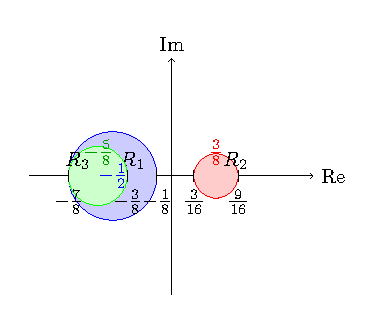
\includegraphics[width=0.7\textwidth]{prueba.pdf} % Adjust width as needed
          \caption{C\'irculos de Gerschgorin para la matriz $A$.}
      \end{figure}
  \end{frame}
    %%%%%%
    \begin{frame}{Ejemplo:}
      \begin{itemize}
        \item La matriz $A$ es no singular ya que el cero esta fuera de los c\'irculos.
        \item Hay un autovalor en $R_2$ y los otros dos est\'an en $R_1 \cup R_3$.
        \item Se puede hacer el mismo an\'alisis para la matriz $A^t$ y obtener otra familia de c\'irculos $R_1',R_2', R_3'$.
        $$
        A^t = \dfrac{1}{16}\left[\begin{array}{ccc}
          -8 & -1 & 2 \\
          -2 & 6 & 2 \\
          4 & 2 & -10      
        \end{array}\right]
        $$
        \item Se tiene que $r_1' = r_1$, $r_2' = r_2$, $r_3' = r_3$. Los discos son:
        \begin{align*}
        R_1' & = \{ z \in \mathbb{C} / |z+1/2|\leq 3/16\}, \Rightarrow -11/16 \leq z \leq -5/16\\
        R_2' & = \{ z \in \mathbb{C} / |z-3/8|\leq 1/4\}, \Rightarrow 1/8 \leq z \leq 5/8\\
        R_3' & = \{ z \in \mathbb{C} / |z+5/8|\leq 3/8\}, \Rightarrow -1 \leq z \leq -1/4
        \end{align*}
      \end{itemize}
    \end{frame}
    %%%%%%
    \begin{frame}{C\'irculos de Gershgorin - $A$ y $A^t$}
      \begin{figure}
        \centering
        \begin{subfigure}{0.48\textwidth}
          \centering
          \begin{tikzpicture}[scale=2]
            % Define the centers and radii of the circles for A
            \def\centerROne{-0.5}
            \def\radiusROne{0.375}
            \def\centerRTwo{0.375}
            \def\radiusRTwo{0.1875}
            \def\centerRThree{-0.625}
            \def\radiusRThree{0.25}
    
            % Draw the axes
            \draw[->] (-1.2,0) -- (1.2,0) node[right] {Re};
            \draw[->] (0,-1) -- (0,1) node[above] {Im};
    
            % Draw the circles
            \draw[blue,fill=blue!20] (\centerROne,0) circle (\radiusROne) node[above right, black] {$R_1$};
            \draw[red,fill=red!20] (\centerRTwo,0) circle (\radiusRTwo) node[above right,black] {$R_2$};
            \draw[green,fill=green!20] (\centerRThree,0) circle (\radiusRThree) node[above left, black] {$R_3$};
    
            % Mark the boundaries of the intervals on the real 
            {\tiny
            \foreach \x/\xtext in {-0.875/-\frac{7}{8}, -0.125/-\frac{1}{8}, 0.1875/\frac{3}{16}, 0.5625/\frac{9}{16}, -0.375/-\frac{3}{8}, -0.375/-\frac{3}{8}}
            {
              \draw (\x,0.05) -- (\x,-0.05) node[below] {$\xtext$};
            }}
    
            % Add some labels for the centers
            \node[blue] at (\centerROne,0) {$-\frac{1}{2}$};
            \node[red] at (\centerRTwo,0.2) {$\frac{3}{8}$};
            \node[green!60!black] at (\centerRThree,0.2) {$-\frac{5}{8}$};
          \end{tikzpicture}
          \caption{C\'irculos de Gershgorin para $A$}          
        \end{subfigure}
        \hfill
        \begin{subfigure}{0.48\textwidth}
          \centering
          \begin{tikzpicture}[scale=2]
            % Define the centers and radii of the circles for At
            \def\centerROne{-0.5}
            \def\radiusROne{0.1875}
            \def\centerRTwo{0.375}
            \def\radiusRTwo{0.25}
            \def\centerRThree{-0.625}
            \def\radiusRThree{0.375}
    
            % Draw the axes
            \draw[->] (-1.2,0) -- (1.2,0) node[right] {Re};
            \draw[->] (0,-1) -- (0,1) node[above] {Im};
    
            % Draw the circles        
            \draw[red,fill=red!20] (\centerRTwo,0) circle (\radiusRTwo) node[above right,black] {$R_2'$};        
            \draw[green,fill=green!20] (\centerRThree,0) circle (\radiusRThree) node[above left, black] {$R_3'$};
            \draw[blue,fill=blue!20] (\centerROne,0) circle (\radiusROne) node[above right, black] {$R_1'$};
    
            % Mark the boundaries of the intervals on the real axis
            {\tiny
              \foreach \x/\xtext in {-1/-1, -0.6875/-\frac{11}{16}, -0.3125/-\frac{5}{16}, 0.125/\frac{1}{8}, 0.625/\frac{5}{8}, -0.25/\;\;\quad\quad-\frac{1}{4}}
            {
              \draw (\x,0.05) -- (\x,-0.05) node[below] {$\xtext$};
            }}
    
            % Add some labels for the centers
            \node[blue] at (\centerROne,0) {$-\frac{1}{2}$};
            \node[red] at (\centerRTwo,0.2) {$\frac{3}{8}$};
            \node[green!60!black] at (\centerRThree,0.2) {$-\frac{5}{8}$};
    
          \end{tikzpicture}
          \caption{C\'irculos de Gershgorin para $A^t$}          
        \end{subfigure}
        \caption{C\'irculos de Gershgorin para $A$ y $A^t$}        
      \end{figure}
    \end{frame}
    %%%%%%
    \begin{frame}{Ejemplo:}
      \begin{itemize}
        \item Se sabe que los autovalores de $A$ y $A^t$ coinciden, por tanto
        la intersecci\'on de $(R_1\bigcup R_2\bigcup R_3) \bigcap (R_1' \bigcup R_2' \bigcup R_3')$ nos da un refinamiento y se obtienen 3
        c\'irculos disjuntos: $C_1, C_2$ y $C_3'$. Se puede concluir que $A$ tiene tres autovalores reales y cada uno de ellos est\'a en los
        intervalos $[-5,-3],[-2,2]$ y $[3,5]$.
      \end{itemize}
    \end{frame}
    %%%%%%
    \begin{frame}
    \begin{eqnarray}
      R_1 = \{ z \in \mathbb{C} / |z-1|\leq 5\}, \Rightarrow -4 \leq z \leq 6\nonumber\\
      R_2 = \{ z \in \mathbb{C} / |z-2|\leq 4\}, \Rightarrow -2 \leq z \leq 6\nonumber
    \end{eqnarray}
    \begin{eqnarray}
       & A^t = \left[\begin{array}{cc}
                                1 & 4 \\
                                5 & 2
                             \end{array}\right] &\nonumber\\
      &C_1 = \{ z \in \mathbb{C} / |z-1|\leq 4\}, \Rightarrow -3 \leq z \leq 5&\nonumber\\
      &C_2 = \{ z \in \mathbb{C} / |z-2|\leq 5\}, \Rightarrow -3 \leq z \leq 7&\nonumber
    \end{eqnarray}
    \end{frame}
    %%%%%%
  \end{document}
